\chapter{Resourcefulness, Leverage, and Scale on the Las Vegas Strip}

This School of Hard Knocks interview, curated by LazyingArt LLC through Video2Book, is not a blackboard lecture in the ordinary sense, but it does have a mathematical spine. The host begins with a city-scale number, then samples several entrepreneurs, and each encounter moves from visible output to hidden mechanism. What we want to preserve is that sequence: first the money field, then the credential, then the origin story, then the operating rule. Where the lecture itself becomes quantitative, we keep the numbers. Where it becomes causal, we translate the causal claims into cautious bookkeeping, update rules, and small schematic models.

\section{Las Vegas as a Money Field}

The lecture opens with a teaser montage: large annual numbers, early millionaire ages, seller identity, and luxury cars. That opening is not yet an argument. It is a promise that the city is dense with commercial evidence. The first stabilizing move is a single scalar:
\begin{equation}
S_{\mathrm{LV}} = 45\times 10^9\,\mathrm{USD}.
\end{equation}
This is the stated amount of money spent in Las Vegas in the past year. Once that number is placed on the table, the city stops being mere backdrop and becomes a field of samples. Each interview is now a local observation inside a much larger flow of capital.

\begin{table}[h]
\centering
\begin{tabular}{|l|l|l|l|l|}
\hline
Case & Vehicle & Years stated & Largest stated figure & Milestone \\
\hline
First Lamborghini & Trading + entrepreneurship & 4 & \$1.5 million & first million at 21 \\
Manufacturing & Medical supplies / paint & not stated & \$5.4 million & age 45 \\
Real estate & Real estate & 20 & tens of millions & long-run asset builder \\
Airbnb & Airbnb & 3 & nearly \$7 million & first million at 20 \\
\hline
\end{tabular}
\caption{Transcript-backed numerical anchors for the four main cases.}
\end{table}

We should notice the host's method already at work. He does not begin with doctrine. He begins with comparability: What do you do? How long? What is the biggest year? How old are you? When did the first million arrive? The point is to certify that the person can speak before the lecture asks why that success happened.

\section{Early Wealth, Delegation, and Earned Scarcity}

The first long case concerns a young entrepreneur driving a Lamborghini. The opening facts are sharp: he trades full time, has been a business owner for about four years, had a best year of \$1.5 million, and made his first million at age twenty-one. The temptation would be to stop there and tell a simple story of precocious market success. The lecture refuses that simplification.

When the host asks how the first million happened, the first answer is market timing: trading during a period when money was easy to make. But the answer does not stay there. The speaker immediately adds the correction: he was not truly at seven figures until he delegated. That is the first major conceptual pivot of the lecture. Luck may create an opening, but durable scale requires distributed capacity.

We can write the transcript's intuition as
\begin{equation}
Y_{\mathrm{team}} = Y_{\mathrm{self}} + \sum_{i=1}^{n} Y_i.
\end{equation}
This is not a literal equation from the speaker; it is our compact way of stating his claim that the founder alone cannot carry every required task. Seven-figure scale appears when the business stops being identical with one person's labor.

The lecture is careful about what makes the team stable. The speaker does not describe delegation as mere task dumping. He names three conditions: treat people very well, pay people very well, and offer opportunities for growth. So the mechanism is not only additive labor. It is also retention, trust, and incentive alignment.

\subsection{Question \& Answer}

\paragraph{Question.} If the first million partly came during an unusually easy market, what turns that temporary opportunity into durable wealth?

\paragraph{Answer.} The lecture's answer is that timing is not enough. A favorable market can produce gains, but a business becomes durable only when its production ceases to be founder-bound. In the transcript, that means delegation, team-building, and the creation of a structure in which other people can reliably do pieces of the work. The deeper claim is that a windfall may begin the story, but organization determines whether the story continues.

The interview then turns from external mechanism to internal formation. The host asks whether the speaker has ever been broke. This is one of the lecture's recurring pressure tests. The answer matters because it reveals whether the present success arose from inherited smoothness or from friction. The speaker says he was raised by a single mother who never gave him anything and made him earn what he had. That answer reframes the earlier success: the key input is not luxury but earned scarcity. The principle is not that deprivation is good in itself. The principle is that being forced to solve one's own immediate problems produces later commercial competence.

\section{Focus, Faith, and Action Before Readiness}

The first interview continues by moving through three layers of discipline: personal focus, theological center, and operational tempo.

First comes focus. The speaker offers an unusual observation: many successful people he knows are married, and he describes marriage as a focusing device. The point is not romance as sentiment, but concentration as strategy. If attention is not fragmented, commercial effort deepens.

Then comes faith. The lecture records the speaker's claim that God must be at the center of everything. He describes asking for a seven-figure business and receiving lessons rather than immediate reward. The business becomes shaky, teams split, things fall out of order, and only afterward does he describe finding stability again. The exact biblical citation in the transcript is internally unstable, but the operational point is clear: he interprets disorder as instruction, not as mere bad luck.

Finally, the lecture arrives at the most portable operational rule in the first case: do not wait for total completeness. Act, then discover what is broken, then repair. We may encode that by the update rule
\begin{equation}
Q_{t+1} = Q_t + \phi\,\Delta_t,
\qquad
\Delta_t = h(A_t),
\end{equation}
where \(A_t\) is action taken at step \(t\), \(\Delta_t\) is the defect set exposed by that action, and \(Q_t\) is the business quality or operating robustness at that stage. The transcript's language is informal, but the logic is unmistakably iterative.

\begin{figure}[h]
\centering
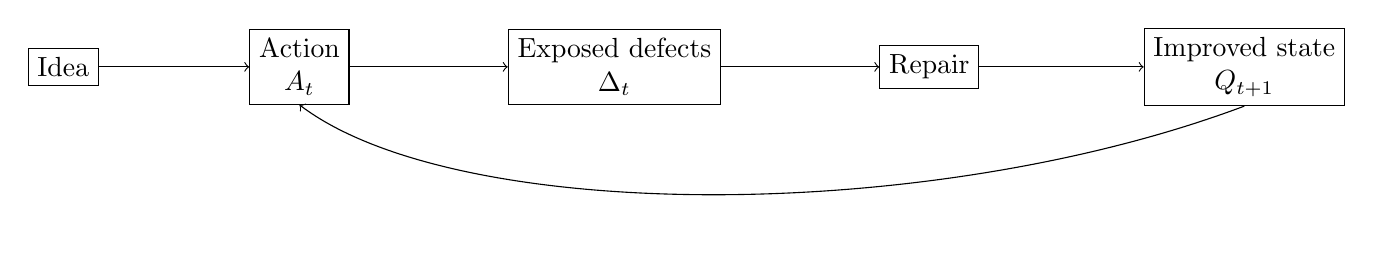
\begin{tikzpicture}[x=1cm,y=1cm]
\node[draw, align=center] (idea) at (0,0) {Idea};
\node[draw, align=center] (act) at (3,0) {Action\\$A_t$};
\node[draw, align=center] (gap) at (7,0) {Exposed defects\\$\Delta_t$};
\node[draw, align=center] (repair) at (11,0) {Repair};
\node[draw, align=center] (quality) at (15,0) {Improved state\\$Q_{t+1}$};

\draw[->] (idea) -- (act);
\draw[->] (act) -- (gap);
\draw[->] (gap) -- (repair);
\draw[->] (repair) -- (quality);
\draw[->] (quality.south) .. controls (11,-2) and (5,-2) .. (act.south);
\end{tikzpicture}
\caption{Transcript-derived action loop: action exposes what planning alone could not reveal, and repair raises the next operating state.}
\end{figure}

\subsection{Question \& Answer}

\paragraph{Question.} Why should we act before the plan is complete?

\paragraph{Answer.} Because in the lecture's logic, incompleteness is not removed by waiting. It is removed by contact with reality. Action reveals hidden defects. Those defects are then repairable. Waiting for perfect readiness suppresses precisely the information needed for improvement. The speaker's slogan is practical rather than philosophical: do not spend two weeks polishing the logo; begin, and let the business teach you what it still lacks.

The host's recap after this interview compresses the whole case toward faith. That recap matters because it tells us what the episode wants the audience to remember, but we should not let the recap erase the earlier mechanism. The full structure of the case is stronger than the recap alone: delegation, earned scarcity, focus, faith, and action.

\section{Legacy, Seller Identity, and Mindset}

The second long case shifts register. We move from young speed to middle-aged scale. The interviewee works in manufacturing, specifically medical supplies and military-grade paint, and says the business did \$5.4 million in its best year. He is forty-five. Here the lecture is no longer asking how somebody moved quickly; it asks what kind of horizon commercial life should have.

The pivotal statement is a proverb: the world becomes a better place when a man plants seeds for future generations and never enjoys the shade himself. The host immediately asks him to break that down. The answer is that one does not hustle merely for oneself. One hustles for the family name, for the line after oneself, for children and grandchildren. The game is long.

That shift matters because it changes the objective function. If the horizon is only personal consumption, then commercial action is short and brittle. If the horizon is generational, then effort can be rational even when the payoff is delayed or partially enjoyed by others. In the lecture's own terms, one works not for James alone but for Dumoulin, not for the individual front but for the name on the back of the jersey.

The same interview then reconnects to an older motif: seller identity. He says he is a seller by nature and that this is why he became an entrepreneur. Here the lecture hints at something like a stable disposition. It is not merely that he learned a sales technique. It is that the commercial relation already felt natural.

\subsection{Question \& Answer}

\paragraph{Question.} Which matters more, mindset or skill set?

\paragraph{Answer.} The interview's answer is clear: mindset. The reason given is portability. A skill set can become rigid and local. A mindset can cross arenas. If a person with the right disposition enters the mail room, he does not remain the mail-room person forever. The claim is not that skill is unnecessary. It is that skill without expansive orientation becomes static, while mindset keeps opening paths into new skill.

This case closes with faith in yet another register: not as explicit business foundation, but as moral compass and ego killer. The lecture likes this pairing. Wealth without ego reduction becomes brittle. Faith, in this speaker's description, keeps ambition from hardening into self-idolatry.

\section{Resourcefulness, Cash Flow, and the Affordability Trap}

The real-estate interview is the analytic center of the lecture. The opening credentials are already enough to command attention: nearly twenty years in real estate and ``tens of millions'' in revenue and net profit. But again the lecture does not stop at scale. It immediately asks about origin.

The key move is subtle and extremely important. The speaker says he did not come from money, but he did come from resources, and then he adds that everyone comes from resources. The true scarcity is not resources; it is the willingness to recognize them and ask for help. We can state the logic with a simple gate:
\begin{equation}
Z_{\mathrm{usable}} = u\,Z_{\mathrm{available}},
\qquad
u\in\{0,1\}.
\end{equation}
Here \(Z_{\mathrm{available}}\) is the stock of accessible helpers, openings, and opportunities, while \(u=1\) means one actually activates those resources by asking. If \(u=0\), the resources remain socially present but economically inert.

\subsection{Question \& Answer}

\paragraph{Question.} Do we lack resources, or do we lack resourcefulness?

\paragraph{Answer.} The lecture answers: usually the latter. The real-estate speaker insists that help was available, but only to the person willing to request it with both humility and nerve. This is a strong and useful distinction. Lack of money is not identical with lack of reachable assistance. The binding constraint may be the refusal to activate what is already nearby.

The next move is equally sharp. The speaker says one cannot save one's way to being rich. The host responds immediately because he recognizes that this is not an aside; it is a replacement of one wealth logic by another. The criticized logic is
\begin{equation}
P \le I-E,
\end{equation}
where \(P\) is the price of the desired object, \(I\) current income, and \(E\) current expenses. The speaker says this is the wrong question. The correct question is not whether the current budget can carry the object, but how income can be expanded and how assets can be made to throw off cash.

So we replace the static budget identity with
\begin{align}
I_{\mathrm{total}} &= I_{\mathrm{labor}} + C_{\mathrm{assets}},\\
C_{\mathrm{monthly}} &= N\,\bar c,\\
R_{\mathrm{annual}} &\approx 12\,C_{\mathrm{monthly}}.
\end{align}
This is the cleanest mathematical compression of the lecture's asset logic. One buys cash-flowing assets, in his preferred case rental properties, and then scales either the number of units \(N\), the per-unit monthly cash flow \(\bar c\), or both.

\begin{figure}[h]
\centering
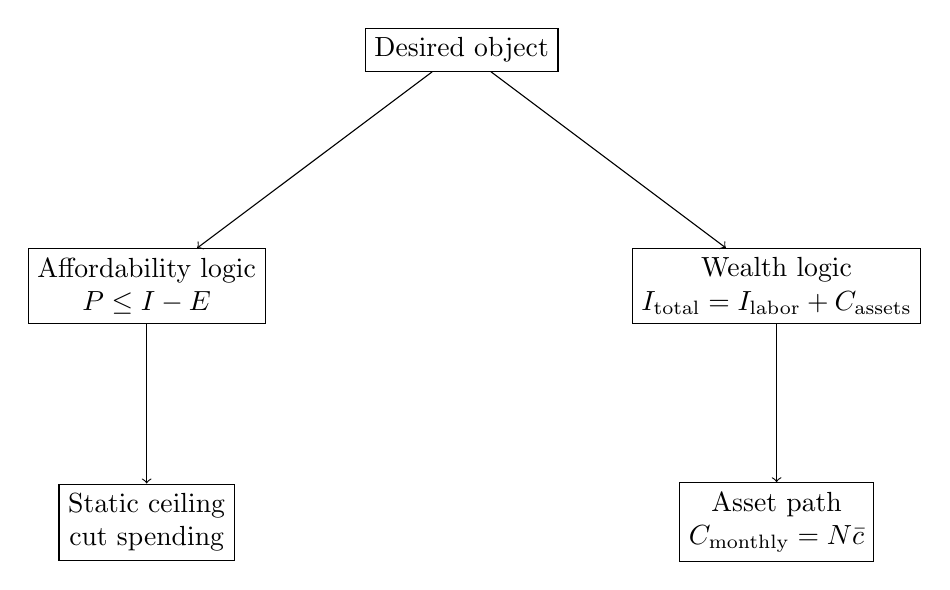
\begin{tikzpicture}[x=1cm,y=1cm]
\node[draw, align=center] (start) at (0,0) {Desired object};
\node[draw, align=center] (left) at (-4,-3) {Affordability logic\\$P \le I-E$};
\node[draw, align=center] (left2) at (-4,-6) {Static ceiling\\cut spending};
\node[draw, align=center] (right) at (4,-3) {Wealth logic\\$I_{\mathrm{total}}=I_{\mathrm{labor}}+C_{\mathrm{assets}}$};
\node[draw, align=center] (right2) at (4,-6) {Asset path\\$C_{\mathrm{monthly}}=N\bar c$};

\draw[->] (start) -- (left);
\draw[->] (start) -- (right);
\draw[->] (left) -- (left2);
\draw[->] (right) -- (right2);
\end{tikzpicture}
\caption{Transcript-derived contrast between the affordability question and the asset-building question.}
\end{figure}

The lecture then broadens into diagnosis. Politics, football, alcohol, and more general distraction are said to keep people broke by washing ambition out of the week. This is not presented as measured sociology, and we should not pretend otherwise. But there is a formal contrast inside it that is worth keeping. The speaker imagines a person in the wilderness with no distractions, no alcohol, no nonsense, and no resources; when one returns six months later, that person has built things. The point is that the default human mode, in his telling, is productive construction once distraction is stripped away. The claim is rhetorical, but the mechanism is recognizable: suppressed agency reappears under concentration and necessity.

The interview ends on cost. Health, family, friend groups, sanity: all are named as sacrificial inputs. That list matters because it prevents the lecture's earlier asset logic from sounding frictionless. Scale has a price.

\section{From Time-for-Money to Scalable Units}

The final major case returns to Airbnb, but now not as teaser bait. It is used as the operational exit of the lecture. The speaker says she was broke, worked as a nanny, was hit by COVID, and found herself at the limit of time-for-money exchange. The mathematical point is immediate:
\begin{equation}
R_{\max}^{\mathrm{wage}} = w\,h_{\max}.
\end{equation}
If income is strictly labor-bound, there is an upper bound. One can like the work and still dislike the ceiling.

That is why the interview turns from pain to leverage. She says she did not want to depend on others, did not want labor hours to determine all income, and eventually learned that business credit existed. Here we should be careful. The lecture provides no rates, leverage ratios, or financing terms. So the valid mathematical content is not a debt model. It is simply the change of architecture: use current income or credit access to create a business that produces income without requiring one more hour of personal labor for every extra dollar.

\subsection{Question \& Answer}

\paragraph{Question.} What can someone at rock bottom do right now?

\paragraph{Answer.} The transcript gives a two-step answer. First, if there is a job, use that income as seed capacity rather than pure consumption. Second, if business credit is available, deploy it toward an income-producing business rather than a consumption item. The lecture's emphasis is not on elegance but on motion: one starts with whatever channel can produce the first paying unit.

Now we can work through the numerical example given by the Airbnb case. The speaker reports an early level of about \$3{,}000 per month, then about \$60{,}000 per month, and then nearly \$400{,}000 in the first calendar year:
\begin{align}
C_0 &\approx \$3{,}000/\text{month},\\
C_1 &\approx \$60{,}000/\text{month},\\
R_{\text{year 1}} &\approx \$400{,}000.
\end{align}
The lecture wants us to hear this not as a miracle but as a scale path. We can make that precise. The average monthly revenue over the first calendar year is
\begin{equation}
\bar C_{\text{year 1}} = \frac{R_{\text{year 1}}}{12} \approx \$33{,}333/\text{month}.
\end{equation}
But if the \$60{,}000 monthly level had been sustained for the entire year, then one would have
\begin{equation}
12\times \$60{,}000 = \$720{,}000,
\end{equation}
which is far above the reported \$400{,}000. Therefore the sixty-thousand-dollar run rate must have been reached after a ramp, not held from the beginning. That is exactly what the lecture means by a numbers game. Scale is not static. It is an accumulation of units, systems, and repeatable wins over time.

The speaker then says Airbnb was simply the first vehicle that worked. She tried many things; this one produced traction first. The lecture's final practical lesson is therefore not ``Airbnb is magical.'' It is that once a vehicle works, one scales it. If purchase is not possible, rent. If ownership is not available yet, control the first unit another way. Then increase \(N\), the number of functioning units, as long as the properties are winners and the cash flow remains positive.

\section{Summary}

The lecture begins with glamour and ends with structure. A city-level spending figure turns Las Vegas into a money field. A young trader explains that luck is not enough without delegation. A manufacturer argues that commercial life should be aimed at legacy rather than the isolated self. A real-estate operator replaces the affordability question with the asset question and says the true scarcity is often resourcefulness, not resources. An Airbnb entrepreneur closes by turning the refusal of wage ceilings into a simple scaling rule.

What remains after the cars and the one-line recaps is a coherent sequence of mechanisms. We move from founder-bound output to team output, from planning to action-feedback, from static budgets to cash-flow assets, and from hourly exchange to scalable units. That is the real payload of the lecture. The visible symbols are absent, but the hidden equations are there.